\chapter{User Environment}
\label{cha:user_environment}

\section{User Environments and Exception Handling}
\par inc/env.h中包含了基本的环境定义。在kern/env.c中,可以看到内核维护了3个全局变量来存储环境。
\begin{itemize}
    \item struct Env *envs = NULL; //ALL environments
    \item struct Env *curenv = NULL; The current env
    \item static struct Env *env\_free\_list; //Free environment list
\end{itemize}
\par jOS开始运行以后,env指针将指向一个存放系统各种环境的Env结构体数组。jOS内核最大支持NENV个同时活动的环境。jOS内核使用env\_free\_list维护所有不同的Env结构体,类似于空闲链表。内核使用curenv来表示当前运行的环境。内核启动前这个变量是NULL。

\subsection{Environment State}
\par Env结构体在inc/env中定义:
\inputCodeSetLanguage{c}
\begin{lstlisting}
struct Env {
    struct Trapframe env_tf;	// Saved registers
    struct Env *env_link;		// Next free Env
    envid_t env_id;			    // Unique environment identifier
    envid_t env_parent_id;		// env_id of this env's parent
    enum EnvType env_type;		// Indicates special system environments
    unsigned env_status;		// Status of the environment
    uint32_t env_runs;		    // Number of times environment has run

    // Address space
    pde_t *env_pgdir;		    // Kernel virtual address of page dir
};
\end{lstlisting}
\par 其中:
\begin{itemize}
    \item env\_tf:定义在inc/trap.h中,用于存放环境停止运行时寄存器的值。切换为内核模式的时候也会保存寄存器的值。
    \item env\_link:指向env\_free\_list中的下一个Env,env\_free\_list空闲链表的第一个env环境。
    \item env\_id:内核储存env\_id环境的父用户环境id。
    \item env\_type:用来特定环境。
    \item env\_status:这个变量可能为以下几种值:
        \begin{itemize}
            \item ENV\_FREE:这个Env是不活跃的,也就是说在env\_free\_list中。
            \item ENV\_RUNNABLE:这个Env正在等待被处理器运行。
            \item ENV\_RUNNING:这个Env结构体代表了正在运行的环境。
            \item ENV\_NOT\_RUNNABLE:当前环境是活跃的但是不准备运行。比如等待其他环境进行进程间通信。
            \item ENV\_DYING:Env是一个僵尸环境,这个环境下一次进入内核的时候会被释放。
        \end{itemize}
    \item env\_pgdir:这个变量存放这个环境的页目录的虚拟地址。
\end{itemize}
\par 类似于Unix,一个jOS环境中结合了``线程''和``地址空间''的概念。线程是由保护寄存器定义的,而地址空间是由env\_pgdir指向的页目录和页表定义。

\subsection{Allocating the Environments Array}
\par 在lab2中修改了mem\_init()内为pages数组分配了空间,而现在需要进一步修改mem\_init()来为Env分配一个相似的结构envs。
\exercise{1}{
    \par 修改kern/pmap.c中的mem\_init()来为envs分配空间并建立映射。这个数组应该正好包含NENV个Env结构。并且这个envs应该映射到用户制度的UENVS,这样用户进程可以读取。可以使用check\_kern\_pgdir()来检查代码是否正确。
}
\begin{exerciseSolution}{1}
    \par 首先是分配数组,在分配pages的代码后添加为envs分配空间的代码:
    \inputCodeSetLanguage{c}
    \begin{lstlisting}
envs = (struct Env*)boot_alloc(NENV*sizeof(struct Env));
memset(envs, 0, NENV*sizeof(struct Env));
    \end{lstlisting}
    \par 在分配完内存空间之后,接下来准备映射。因此在对于pages的映射之后对envs进行映射,添加如下代码:
    \begin{lstlisting}
boot_map_region(kern_pgdir, UENVS, PTSIZE, PADDR(envs), PTE_U);
    \end{lstlisting}

    \par 修改完成以后,重新编译运行,结果如图\ref{fig:lab3/exercise1_1}所示。可以看到,显示check\_kern\_pgdir() succeeded!,也就是说exercise1实验成功。
    \begin{figure}[htb]
        \centering
        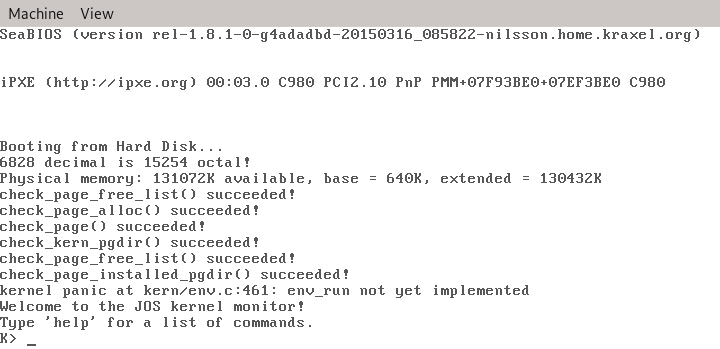
\includegraphics[width=0.8\linewidth]{lab3/exercise1_1.png}
        \caption{修改mem\_init后的运行结果}
        \label{fig:lab3/exercise1_1}
    \end{figure}
    \FloatBarrier
\end{exerciseSolution}

\subsection{Creating and Running Environments}
\par 现在需要完善kern/env.c使之能够运行一个用户环境。由于没有文件系统,因此必须将内核设置为能够加载内核中的静态二进制程序映像文件。
\par Lab3里面的GNUMakefile文件在obj/user目录下生成了一系列二进制文件。通过kern/Makefrag能够将这些二进制文件直接链接到可执行文件中。通过链接器中的-b binary选项能够使这些文件被作为二进制文件链接到内核之后。
\exercise{2}{
    \par 在env.c中,完成以下函数:
    \begin{itemize}
        \item env\_init()
            \par 初始化所有在envs数组中的Env结构,并将其加入env\_free\_list中。此外还需要调用env\_init\_percput来配置段式内存管理硬件来将所有的分段分为0级(内核)以及3级(用户)。
        \item env\_setup\_vm()
            \par 分配页目录,初始化用户环境地址空间中和内核相关的部分。
        \item region\_alloc()
            \par 为用户环境分配物理空间。
        \item load\_icode()
            \par 像boot loader一样分析一个ELF文件,并将它的内容加载到用户环境下。
        \item env\_create()
            \par 使用env\_alloc和load\_icode函数分配空间并加载一个ELF文件到用户环境中。
        \item env\_run()
            \par 在用户模式下开始一个用户环境。
    \end{itemize}
}
\begin{exerciseSolution}{2}
    \par 对于env\_init函数而言,遍历envs数组中的Env结构体,把每一个Env的end\_id置0。实现的env\_init的代码如下:
    \begin{lstlisting}
void env_init(void) {
    int counter;
    env_free_list = NULL;
    for (counter = NENV - 1; counter >= 0; --counter) {
        envs[counter].env_id = 0;
        envs[counter].env_status = ENV_FREE;
        envs[counter].env_link = env_free_list;
        env_free_list = &envs[counter];
    }
    // Per-CPU part of the initialization
    env_init_percpu();
}
    \end{lstlisting}

    \par 然后填写env\_setup\_vm部分。env\_setup\_vm的函数的作用是初始化新的用户环境页目录表,但是只设置夜幕里表中和内核相关的页目录,而不映射用户目录。因此可以使用kern\_pgdir来设置env\_pgdir中的内容。最终补充的代码如下:
    \begin{lstlisting}
++p->pp_ref;
e->env_pgdir = (pde_t *)page2kva(p);
memcpy(e->env_pgdir, kern_pgdir, PGSIZE);
    \end{lstlisting}

    \par 接下来补充为用户环境分配len字节的空间的函数,然后映射到环境中的虚拟地址va,根据提示,va向下对齐,va+len向上对齐。
    \begin{lstlisting}
static void region_alloc(struct Env *e, void *va, size_t len) {
    struct PageInfo *page = NULL;
    va = ROUNDDOWN(va, PGSIZE);
    void *end = (void *)ROUNDUP(va + len, PGSIZE);
    for (; va < end; va += PGSIZE) {
        if (!(page = page_alloc(ALLOC_ZERO)))
            panic("region_alloc: alloc failed.");
        if (page_insert(e->env_pgdir, page, va, PTE_U | PTE_W))
            panic("region_alloc: page mapping failed.");
    }
}
    \end{lstlisting}

    \par load\_icode需要加载ELF二进制到用户内存。参考boot/main.c中的boot loader加载内核到内存,首先验证ELF文件的合法性,然后加载ph->
p\_type = ELF\_PROG\_LOAD的字段,在加载前需要注意使用lcr3切换到用户态的页目录,否则不能够正确的加载到用户内存空间。在加载完成并将多余位清零后,映射初始栈的一个页,最终完成的代码如下:
    \begin{lstlisting}
static void load_icode(struct Env *e, uint8_t *binary) {
    struct Elf *elf_header = (struct Elf *)binary;
    if (elf_header->e_magic != ELF_MAGIC)
        panic("load_icode: illegal ELF format.");
    lcr3(PADDR(e->env_pgdir));
    struct Proghdr *ph = (struct Proghdr *)((uint8_t *)(elf_header) + elf_header->e_phoff);
    struct Proghdr *eph = ph + elf_header->e_phnum;
    for (; ph < eph; ++ph) {
        if (ph->p_type == ELF_PROG_LOAD) {
            region_alloc(e, (void *)ph->p_va, ph->p_memsz);
            memmove((void *)ph->p_pa, binary + ph->p_offset, ph->p_filesz);
            memset((void *)(ph->p_pa + ph->p_filesz), 0, ph->p_memsz - ph->p_filesz);
        }
    }
    e->env_tf.tf_eip = elf_header->e_entry;
    lcr3(PADDR(kern_pgdir));
    region_alloc(e, (void *)(USTACKTOP - PGSIZE), PGSIZE);
}
    \end{lstlisting}

    \par 对于env\_create首先使用env\_alloc创建一个env,然后调用load\_icode来加载elf二进制镜像,最后设置env\_type。值得注意的是env的父id应该设置为0,其实现如下:
    \begin{lstlisting}
void env_create(uint8_t *binary, enum EnvType type) {
    struct Env *environment;
    if(env_alloc(&environment, 0))
        panic("env_create: env_alloc failed.");
    load_icode(environment, binary);
    environment->env_type = type;
}
    \end{lstlisting}

    \par 对于env\_run而言,首先切换判断当前环境是否为空,环境状态是否为ENV\_RUNNING,如果是则将环境设置为ENV\_RUNNABLE,然后将curenv设置为当前环境。设置状态ENV\_RUNNING,更新env\_runs计数器后切换到它的地址空间。使用env\_pop\_tf换源环境寄存器然后进入用户模式。实现的代码如下:
    \begin{lstlisting}
void env_run(struct Env *e) {
    if(curenv && curenv->env_status == ENV_RUNNING)
        curenv->env_status = ENV_RUNNABLE;
    curenv = e;
    curenv->env_status = ENV_RUNNING;
    ++curenv->env_runs;
    lcr3(PADDR(curenv->env_pgdir));
    env_pop_tf(&curenv->env_tf);
}
    \end{lstlisting}
\end{exerciseSolution}

\par 用户环境的代码被调用前,操作系统一共按顺序执行了以下几个函数:
\begin{itemize}
    \item start (kern/entry.S)
    \item i386\_init (kern/init.c)
        \begin{itemize}
            \item cons\_init
            \item mem\_init
            \item env\_init
            \item trap\_init (still incomplete at this point)
            \item env\_create
            \item env\_run
                \begin{itemize}
                    \item env\_pop\_tf
                \end{itemize}
        \end{itemize}
\end{itemize}
\par 完成上述函数的代码后重新编译运行,系统会进入用户空间并且开始执行hello程序,直到系统调用int指令。这个指令不能成功执行,因为jOS还没有设置相关硬件来实现从用户态向内核态转换的功能。当CPU发现它不能处理这种中断时会触发一个异常,然后发现这个异常也无法处理,直到产生第三个异常,但仍旧不能解决,因此将其叫做"triple fault"。我们可以使用调试器检查我们是否进入了用户模式。使用make qemu-gdb并在env\_pop\_tf处设置一个断点,然后单步执行,处理器会在执行完iret指令以后进入用户模式。该进入用户模式的第一条指令是一个cmp指令。然后使用b *0x...设置一个在obj/user/hello.asm中的断点中的sys\_cputs函数的int \$0x30处。这个int指令是一个系统调用,用来向控制台输出一个字符。如果你的程序不能运行到int指令说明程序有错误。
\par 按照上述过程进行调试,程序停止在了int \$0x30处,如图\ref{fig:lab3/exercise2_1}所示。说明程序功能正常。
\begin{figure}[htb]
    \centering
    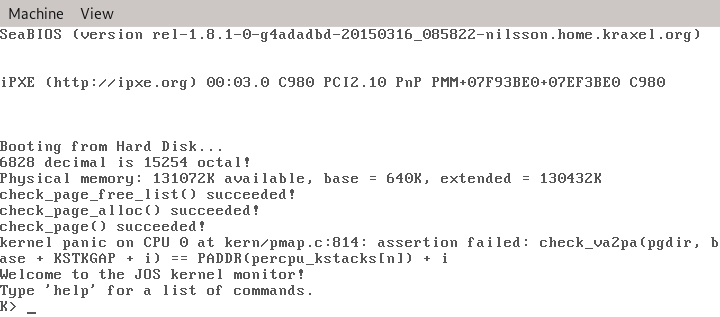
\includegraphics[width=0.9\linewidth]{lab3/exercise2_1.png}
    \caption{程序停止在int \$0x30处}
    \label{fig:lab3/exercise2_1}
\end{figure}

\subsection{Handling Interrupts and Exceptions}
\par 现在需要一个异常处理及系统调用处理机制来使系统从用户态切换到内核态。
\exercise{3}{
    \par 阅读\textit{Chapter 9, Exceptions and Interrupts }\footnote{\url{https://pdos.csail.mit.edu/6.828/2017/readings/i386/c09.htm}}
}
%\begin{exerciseSolution}{3}
%    \par 从文中可以知道,中断分为可屏蔽中断以及不可屏蔽中断;异常分为处理器检测异常以及程序触发的异常。通过NMI、IF、RF以及修改SS可以使能或屏蔽中断。中断描述符表储存中断处理程序的入口地址,而中断的处理流程如图\ref{fig:lab3/exercise3_1}所示,通过IDT与GDT共同决定用于处理的程序。
%    \begin{figure}[htb]
%        \centering
%        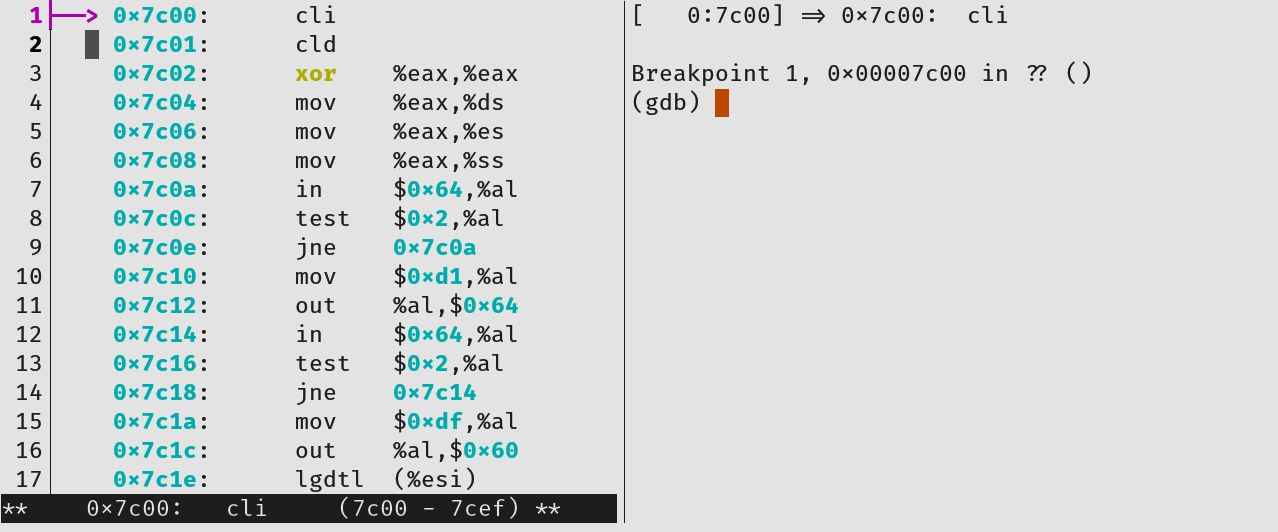
\includegraphics[width=0.6\linewidth]{lab3/exercise3_1.png}
%        \caption{中断处理流程}
%        \label{fig:lab3/exercise3_1}
%    \end{figure}
%\end{exerciseSolution}

\subsection{Basics of Protected Control Transfer}
\par 异常和中断都是保护控制转移,让处理器从用户模式切换到内核模式。这样用户代码不会对内核造成任何影响。在intel处理器中,中断通常是外部设备引起的异步的保护控制转移,而异常则是由当前运行的代码引起的同步的保护控制转移。
\par 为了能够保证这些控制转移真的能被保护,处理器的中断/异常机制通常为用户态代码无权选择内核代码的执行起点,处理器只有在某些条件下才能进入内核态。在x86上,有2中机制配合来提供这种保护:
\begin{enumerate}
    \item 中断向量表:
        \par 处理器保证撞断和异常只能导致内核进入一些预先定好的入口。x86处理器可以有最多256个不同的中断和异常,而每一个都对应一个唯一的中断向量。一个中断向量的值是根据中断的来源决定的。CPU将使用这个向量作为中断向量表的索引,而这个表又是内核设置的。通过表项处理器会加载:
        \begin{itemize}
            \item 加载到EIP寄存器的值,也就是指向处理这种类型异常的内核代码指针。
            \item 加载到CS寄存器的值,包含特权级别0\textasciitilde 1。
        \end{itemize}
    \item 任务状态段:
        \par 处理器需要存放中断异常发生之前的旧的处理器状态,包括原EIP和CS值,以在中断处理之后能够还原到之前的状态。保存的这个位置必须要受到保护,不能随意被修改。
        \par 因此,处理西在处理中断时会导致特权级别由用户转级为内核级,将堆切换到内核内存中。处理器将SS, ESP, EFLAGS, CS, EIP和可选的错误码压入堆栈中,然后从中断描述符中加载CS和EIP,设置ESP和SS指向新的堆栈。
\end{enumerate}

\subsection{Types of Exceptions and Interrupts}
\par 所有的x86处理器内部产生的议程向量是0\textasciitilde 31之间的整数,也映射到了IDT的0\textasciitilde 31项。大于31的项只被软件中断所使用,也就是说可以被int触发,或者是异步的硬件中断。
\par 这一节将要扩展jOS的功能使之能够处理0\textasciitilde 31号的内部异常。下一节会让jOS处理48号软件中断。

\subsection{An Example}
\par 在这个例子中,假设处理器遇到了除0的问题。
\begin{enumerate}
    \item 处理器切换到TSS的SS0和ESP0对应的堆栈,在jOS中,这两个字段是GD\_KG和KSTACKTOP。
    \item 处理器将异常参数压入内核堆栈,并放在KSTACKTOP中。
        \inputCodeSetLanguage{bash}
        \begin{lstlisting}[numbers=none]
+--------------------+ KSTACKTOP
| 0x00000 | old SS   |     " - 4
|      old ESP       |     " - 8
|     old EFLAGS     |     " - 12
| 0x00000 | old CS   |     " - 16
|      old EIP       |     " - 20 <---- ESP
+--------------------+
        \end{lstlisting}
   \item 由于处理器错误在x86上是0号中断向量,因此去读IDT的第0项并设置CS:EIP指向中断处理程序。
   \item 处理函数接过控制权并处理异常。
\end{enumerate}
\par 对于确定类型的x86异常,除了上面标准的5个压栈元素外还有一个错误码。当处理器将错误码压栈时,栈是这样的:
\begin{lstlisting}[numbers=none]
+--------------------+ KSTACKTOP
| 0x00000 | old SS   |     " - 4
|      old ESP       |     " - 8
|     old EFLAGS     |     " - 12
| 0x00000 | old CS   |     " - 16
|      old EIP       |     " - 20
|     error code     |     " - 24 <---- ESP
+--------------------+
\end{lstlisting}

\subsection{Nested Exceptions and Interrupts}
\par 处理器在内核模式和用户模式都可以处理异常和中断。但是当内核从用户态进入内核态的时候,x86处理器会在压入旧的寄存器之前自动切换栈并通过IDT触发异常处理。如果当中断或异常发生时处理器已经在内核态了,那么CPU会在同一个栈上压入更多的值。这样,内核就能够处理嵌套中断;了。如果处理器已经在内核模式且正在处理嵌套异常,就不会保存SS和ESP寄存器,因此堆栈如下:
\begin{lstlisting}[numbers=none]
+--------------------+ <---- old ESP
|     old EFLAGS     |     " - 4
| 0x00000 | old CS   |     " - 8
|      old EIP       |     " - 12
+--------------------+
\end{lstlisting}
\par 如果处理器在内核模式处理异常,但栈空间不足,不能将旧的状态压入堆栈,那么处理器之后就不能恢复,只能重启。内核应该被设计为不允许这种事情发生。

\subsection{Setting Up the IDT}
\par 现在可以设置IDT表并处理JOS的内部异常了(中断向量0\textasciitilde 31)。最终需要实现的代码效果如下:
\inputCodeSetLanguage{bash}
\begin{lstlisting}[numbers=none]
       IDT              trapentry.S       trap.c
+----------------+
|   &handler1    |---> handler1:        trap (struct Trapframe *tf)
|                |        // do stuff    {
|                |        call trap        // handle the exception/interruput
|                |        // ...         }
+----------------+
|   &handler2    |---> handler2:
|                |       // do stuff
|                |       call trap
|                |       // ...
+----------------+
        ...
+----------------+
|   &handlerX    |---> handlerX:
|                |        // do stuff
|                |        call trap
|                |        // ...
+----------------+
\end{lstlisting}
\par 每一个中断或者异常结构都有它的中断处理函数,定义在trapentry.S中。trap\_init()初始化IDT表。每个处理函数都应该构建一个在Trapframe堆栈上的结构体,并调用trap()函数指向它。trap()则处理异常/中断。

\exercise{4}{
    \par 编辑trap.S以及trap.c并实现上述功能。对于每一个定义在inc/trap.h中的trap,都应该有一个函数入口应该被加在trapentry.S中。应该提供一个\_alltraps供TRAPHANDLER宏引用。要初始化idt表需要修改trap\_init函数,使表中的每一项指向定义在 trapentry.S 中的入口指针。实现的\_alltraps函数应该:
    \begin{enumerate}
        \item 将值压入堆栈,使堆栈看起来像一个Trapframe
        \item 加载GD\_KD进入\%ds以及\%es
        \item 使用pusl \%esp给Trapframe传递指针,作为trap()的参数
        \item 调用trap
    \end{enumerate}
}
\begin{exerciseSolution}{4}
    \par 首先,trapentry.S 中的宏定义TRAPHANDLER以及TRAPHANDLER\_NOEC定义了发生中断或异常时用于初始处理的函数。因为有些中断有错误码,有些没有,因此需要两个函数。通过参考\textit{80386 Programmer’s Manual 9.10 Error Code Summary}\footnote{\url{https://pdos.csail.mit.edu/6.828/2016/readings/i386/s09_10.htm}}可以知道哪些中断有错误码。因此trapentry.S修改如下:

\inputCodeSetLanguage{[x86masm]Assembler}
\begin{lstlisting}
TRAPHANDLER_NOEC(handler_divide,  T_DIVIDE)
TRAPHANDLER_NOEC(handler_debug,   T_DEBUG)
TRAPHANDLER_NOEC(handler_nmi,     T_NMI)
TRAPHANDLER_NOEC(handler_brkpt,   T_BRKPT)
TRAPHANDLER_NOEC(handler_oflow,   T_OFLOW)
TRAPHANDLER_NOEC(handler_bound,   T_BOUND)
TRAPHANDLER_NOEC(handler_illop,   T_ILLOP)
TRAPHANDLER_NOEC(handler_device,  T_DEVICE)
TRAPHANDLER_NOEC(handler_simderr, T_SIMDERR)
TRAPHANDLER_NOEC(handler_fperr,   T_FPERR)
TRAPHANDLER_NOEC(handler_mchk,    T_MCHK)
TRAPHANDLER_NOEC(handler_syscall, T_SYSCALL)
TRAPHANDLER(handler_dblflt, T_DBLFLT)
TRAPHANDLER(handler_tss,    T_TSS)
TRAPHANDLER(handler_segnp,  T_SEGNP)
TRAPHANDLER(handler_stack,  T_STACK)
TRAPHANDLER(handler_gpflt,  T_GPFLT)
TRAPHANDLER(handler_pgflt,  T_PGFLT)
TRAPHANDLER(handler_align,  T_ALIGN)

_alltraps:
    pushl %ds
    pushl %es
    pushal
    movw $GD_KD, %eax
    movw %ax, %ds
    movw %ax, %es
    pushl %esp
    call trap
\end{lstlisting}
\par 然后在trap.c中完成trap\_init,对于系统的IDT表进行初始化:
\inputCodeSetLanguage{c}
\begin{lstlisting}
void handler_divide();
void handler_debug();
void handler_nmi();
void handler_brkpt();
void handler_oflow();
void handler_bound();
void handler_illop();
void handler_device();
void handler_simderr();
void handler_fperr();
void handler_mchk();
void handler_syscall();
void handler_dblflt();
void handler_tss();
void handler_segnp();
void handler_stack();
void handler_gpflt();
void handler_pgflt();
void handler_align();

void
trap_init(void)
{
    extern struct Segdesc gdt[];

    SETGATE(idt[T_DIVIDE],  0, GD_KT, handler_divide,  0);
    SETGATE(idt[T_DEBUG],   0, GD_KT, handler_debug,   0);
    SETGATE(idt[T_NMI],     0, GD_KT, handler_nmi,     0);
    SETGATE(idt[T_BRKPT],   0, GD_KT, handler_brkpt,   3);
    SETGATE(idt[T_OFLOW],   0, GD_KT, handler_oflow,   0);
    SETGATE(idt[T_BOUND],   0, GD_KT, handler_bound,   0);
    SETGATE(idt[T_ILLOP],   0, GD_KT, handler_illop,   0);
    SETGATE(idt[T_DEVICE],  0, GD_KT, handler_device,  0);
    SETGATE(idt[T_SIMDERR], 0, GD_KT, handler_simderr, 0);
    SETGATE(idt[T_FPERR],   0, GD_KT, handler_fperr,   0);
    SETGATE(idt[T_MCHK],    0, GD_KT, handler_mchk,    0);
    SETGATE(idt[T_SYSCALL], 0, GD_KT, handler_syscall, 3);
    SETGATE(idt[T_DBLFLT],  0, GD_KT, handler_dblflt,  0);
    SETGATE(idt[T_TSS],     0, GD_KT, handler_tss,     0);
    SETGATE(idt[T_SEGNP],   0, GD_KT, handler_segnp,   0);
    SETGATE(idt[T_STACK],   0, GD_KT, handler_stack,   0);
    SETGATE(idt[T_GPFLT],   0, GD_KT, handler_gpflt,   0);
    SETGATE(idt[T_PGFLT],   0, GD_KT, handler_pgflt,   0);
    SETGATE(idt[T_ALIGN],   0, GD_KT, handler_align,   0);

    // Per-CPU setup
    trap_init_percpu();
}
\end{lstlisting}
\par 完成后使用make grade进行测试,可以发现divzero,softint以及badsegment测试通过,如图\ref{fig:lab3/exercise4_1}所示,说明IDT初始化正确。
\begin{figure}[htb]
    \centering
    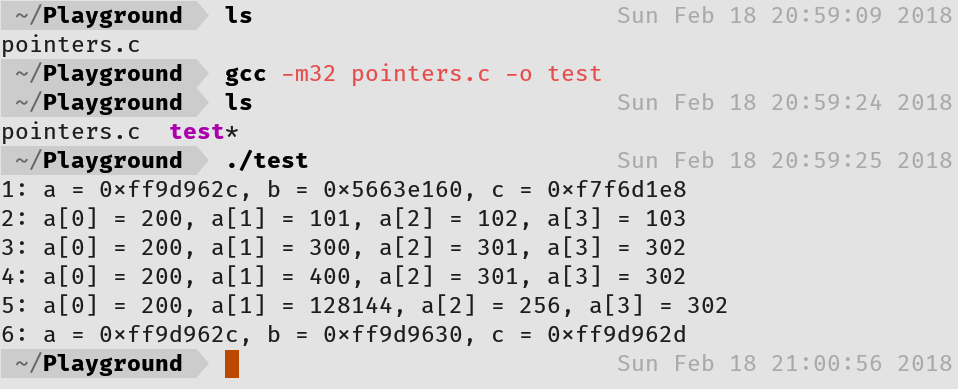
\includegraphics[width=0.8\linewidth]{lab3/exercise4_1.png}
    \caption{使用make grade进行测试}
    \label{fig:lab3/exercise4_1}
\end{figure}
\FloatBarrier
\end{exerciseSolution}

\begin{questionEnv}
    \begin{enumerate}
        \item 对于每一个中断/异常都设置一个独立的处理函数的意义是什么?
        \item 你做了让user/softint正确执行的工作吗?grade script希望它产生一个general protection falt(trap 13),但是softint中为int \$14。为什么产生了中断向量13?如果系统允许int \$14调用kernel page fault处理函数?
    \end{enumerate}
\end{questionEnv}
\begin{answer}
    \begin{enumerate}
        \item 因为不同的中断可能需要不同的处理方式,比如有些中断需要返回,有些中断则不需要,还有些中断需要做额外的工作。
        \item 应为当先系统在用户态,而int为特权级别为0的指令,此时不能直接调用int指令,会引发general protection exception。如果允许int \$14处理,那么会导致用户态程序可能得到0级特权,造成保护失效。
    \end{enumerate}
\end{answer}

\section{Page Faults, Breakpoints Exceptions, and System Calls}
\subsection{Handling Page Faults}
\par 当处理器产生一个缺页异常时,它会将因此缺页异常的线性地址(虚拟的)存入CR2中。在trap.c中我们提供了一个特殊的函数page\_fault\_handler()用于处理缺页异常。
\exercise{5}{
    \par 修改trap\_dispatch函数使系统能够把缺页异常分发到page\_fault\_handler上。修改完成后运行make grade应该可以成功通过faultread, faultreadkernel, faultwrite, 以及faultwritekernel检查。
}
\begin{exerciseSolution}{5}
    \par trap\_dispatch是一个分发函数,通过Trapframe指针tf中的tf\_trapno来判断这个中断是什么中断。而在这一个exercise中,如果中断是缺页中断则调用page\_fault\_handler函数。考虑到之后可能要添加的中断类型,在trap\_dispatch中添加的代码如下:
    \inputCodeSetLanguage{c}
    \begin{lstlisting}
switch(tf->tf_trapno){
    case T_PGFLT:
        page_fault_handler(tf);
        break;
}
    \end{lstlisting}
    \par 重新编译运行后,通过了题目描述中的4个测试,如图\ref{fig:lab3/exercise5_1}所示。说明这部分代码实现成功。
    \begin{figure}[htb]
        \centering
        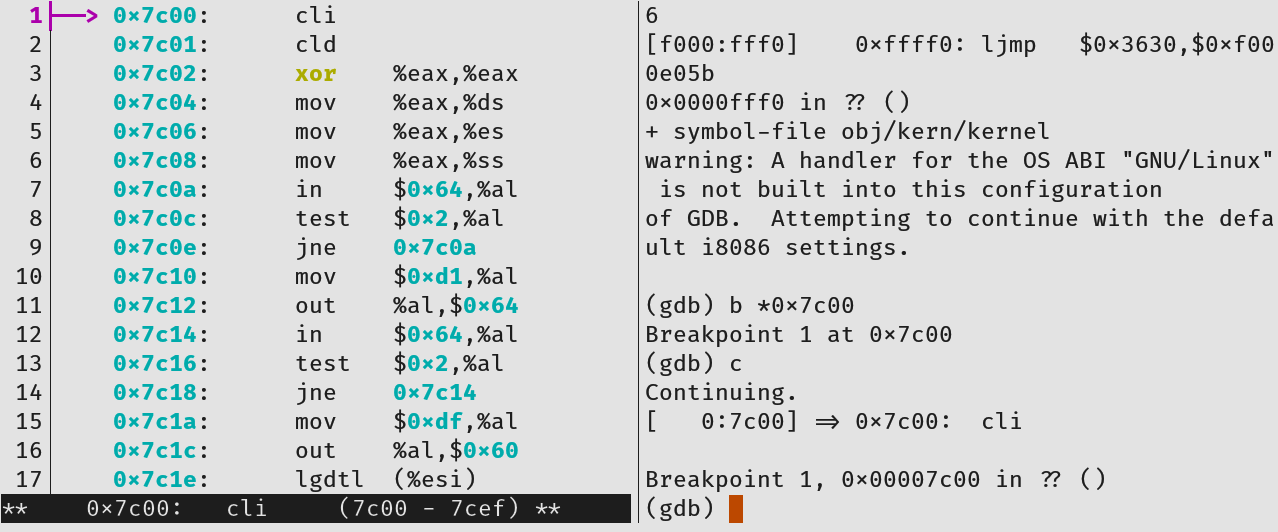
\includegraphics[width=0.8\linewidth]{lab3/exercise5_1.png}
        \caption{重新编译运行后的make grade输出}
        \label{fig:lab3/exercise5_1}
    \end{figure}
\end{exerciseSolution}

\subsection{The Breakpoint Exception}
\par 异常编号为3的断点异常能够让调试器给程序加上断点,也就是将要加断点的语句用一个int3指令替换,然后在执行到int3时触发中断。在jOS中需要将这个中断变为任何用户环境都能调用的伪系统调用。
\exercise{6}{
    \par 修改trap\_dispatch,使断点异常发生时能够调用kernel monitor。修改完成后重新make grade应该能够通过breakpoint测试。
}
\begin{exerciseSolution}{6}
    \par 与exercise 5类似,但是这里处理的是T\_BRKPT。调用kernel monitor需要使用kern/monitor.c中的monitor函数。修改后的trap\_dispatch中的前半部分内容如下:
    \inputCodeSetLanguage{c}
    \begin{lstlisting}
switch(tf->tf_trapno){
    case T_PGFLT:
        page_fault_handler(tf);
        break;
    case T_BRKPT:
        monitor(tf);
        break;
}
    \end{lstlisting}
    \par 修改完成后,成功通过breakpoint测试,如图\ref{fig:lab3/exercise6_1}所示。
    \begin{figure}[htb]
        \centering
        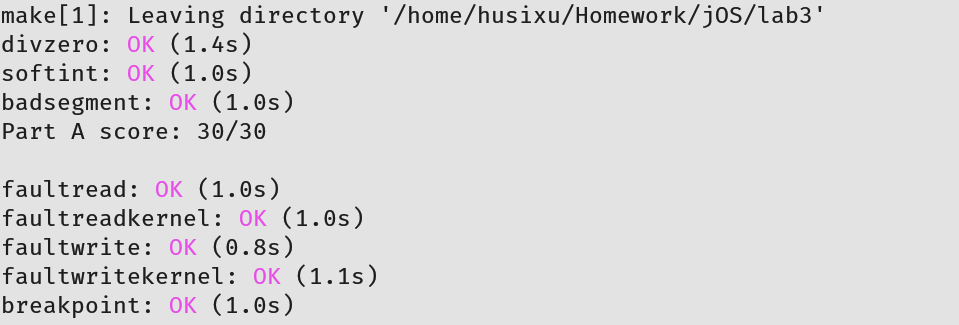
\includegraphics[width=0.8\linewidth]{lab3/exercise6_1.png}
        \caption{程序通过breakpoint测试输出}
        \label{fig:lab3/exercise6_1}
    \end{figure}
\end{exerciseSolution}

\begin{questionEnv}
    \begin{enumerate}
        \setcounter{enumi}{2}
        \item breakpoint exeception测试用例会征程一个breakpoint 异常或者general protection 错误,依赖于如何初始化IDT中的breakpoint entry。为什么?要怎么做才能让breakpoint exception正常工作?怎样的错误设置会导致触发general protection error?
        \item 这些机制有什么意义?尤其是对于user/softint中的测试程序而言?
    \end{enumerate}
\end{questionEnv}
\begin{answer}
    \begin{enumerate}
        \setcounter{enumi}{2}
        \item 如果在IDT中设置breakpoint exception时将DPL字段设置为0则会触发breakpoint exception,设置为3则会触发general protection exception。DPL字段为段描述符优先级,如果当前程序为用户态但是尝试调用内核态的指令的时候就会触发general protection exception。只有当前程序的优先级小于或等于段描述符优先级才能触发正确的breakpoint exception。
        \item 这些机制保证用户环境不能随意访问内核态的代码和内存,保护内核不受用户程序的破坏。
    \end{enumerate}
\end{answer}

\subsection{System calls}
\par 用户程序会要求内核通过系统调用的方式帮其完成一些任务。当用户程序触发系统调用时,处理器进入内核态并保存用户的处理状态。内核处理完成后返回用户程序,但具体的细节随系统的不同而不同。
\par jOS使用int来处理系统调用。特别的,使用int \$0x30作为系统调用中断。常量T\_SYSCALL就是0x30。0x30不能被外部硬件产生,因此没有任何歧义。
\par 应用程序会把系统调用和参数放到寄存器中,通过这种方法内核就不需要查询用户程序的堆栈了。系统调用号存放到\%eax中,参数则存放在 \%edx, \%ecx, \%ebx, \%edi, 和 \%esi中。返回值存放到\%eax@s中。lib/syscall.c中已有了触发系统调用的方法。
\exercise{7}{
    \par 通过编辑kern/trapentry.S以及kern/trap.c的trap\_init(),给T\_SYSCALL添加一个中断向量处理函数。同时trap\_dispatch也需要被修改,通过调用syscall的方法来处理系统调用。最后,需要在kern/syscall.c中首先实现syscall函数。如果系统调用号不合法,需要syscall返回-E\_INVAL。
    \par 通过make run-hello运行user/hello,qemu应该打印处hello, world,并触发一个page fault。并且make grade应该能够通过testbss测试。
}
\begin{exerciseSolution}{7}
    \par 在用户态执行系统调用时,首先产生了中断30,因此在kern/trapentry.S中添加一个处理函数声明TRAPHANDLER\_NOEC(handler\_syscall, T\_SYSCALL),并在trap\_init中添加handler\_syscall的声明以及在trap\_init中通过SETGATE(idt[T\_SYSCALL], 0, GD\_KT, t\_syscall, 3);将其注册到IDT,这些在exercise 5中已经完成,此时系统已经能够正确捕捉int 30了。
    \par 观察lib/syscall.c的syscall,发现其就是执行了int指令并取回了返回值,而对于这条int指令的处理,则是在kern/syscall.c中进行的。首先,完成kern/trap.c中对于中断的分发,也就是在switch中加入如下几行:
    \inputCodeSetLanguage{c}
    \begin{lstlisting}
case T_SYSCALL:
    tf->tf_regs.reg_eax = syscall(
            tf->tf_regs.reg_eax,
            tf->tf_regs.reg_edx,
            tf->tf_regs.reg_ecx,
            tf->tf_regs.reg_ebx,
            tf->tf_regs.reg_edi,
            tf->tf_regs.reg_esi);
    break;
    \end{lstlisting}
    \par 然后在kern/syscall.c中完成对于syscall的实现,从而完成对于整个int指令的调用:
    \begin{lstlisting}
int32_t syscall(uint32_t syscallno, uint32_t a1,
        uint32_t a2, uint32_t a3, uint32_t a4, uint32_t a5) {
    switch (syscallno) {
        case SYS_cputs:
            sys_cputs((char *)a1, a2);
            return 0;
        case SYS_cgetc:
            return sys_cgetc();
        case SYS_getenvid:
            return sys_getenvid();
        case SYS_env_destroy:
            return sys_env_destroy(a1);
        default:
            return -E_INVAL;
    }
}
    \end{lstlisting}
    \par 填写完成后,重新编译并运行qemu,输出hello world并触发缺页中断。如图\ref{fig:lab3/exercise7_1}所示。
    \begin{figure}[htb]
        \centering
        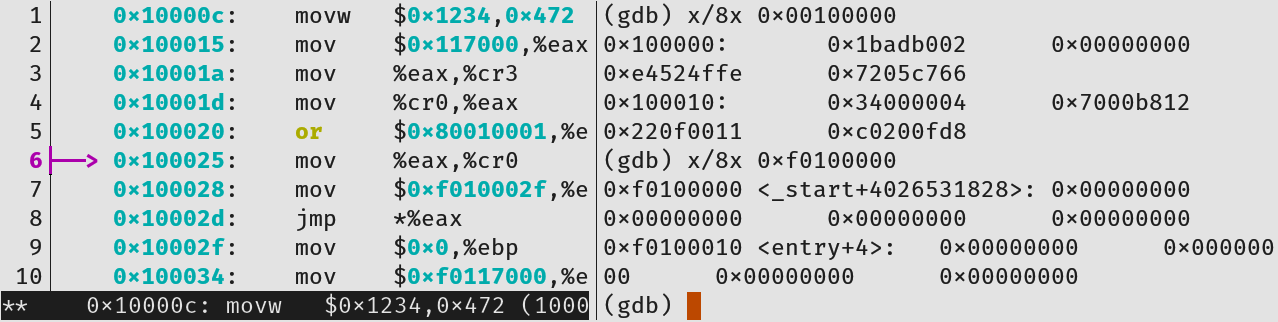
\includegraphics[width=0.8\linewidth]{lab3/exercise7_1.png}
        \caption{输出hello world并触发缺页中断}
        \label{fig:lab3/exercise7_1}
    \end{figure}
    \par 运行make grade,成功通过testbss测试,如图\ref{fig:lab3/exercise7_2}所示,说明系统调用实现成功。
    \begin{figure}[htb]
        \centering
        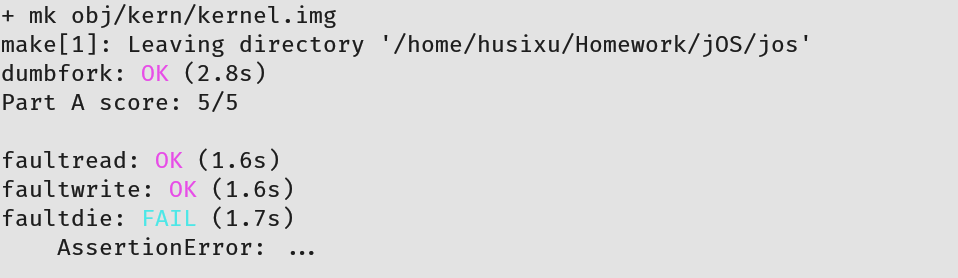
\includegraphics[width=0.8\linewidth]{lab3/exercise7_2.png}
        \caption{成功通过testbss测试}
        \label{fig:lab3/exercise7_2}
    \end{figure}
\end{exerciseSolution}

\subsection{User-mode startup}
\par 用户模式开始运行的地方是lib/entry.S。在该文件中首先进行一些设置,然后调用libmain。应该修改libmain()来初始化全局指针thisenvz指向envs数组中的Env结构体。
\par 然后libmain调用main,也就是user/hello.c中被调用的函数。在之前的实验中发现hello.c只能打印hello world并报出page fault异常,而其原因就是this->env\_id语句。如果正确初始化了thisenv就不会报错了。
\exercise{8}{
    \par 补全用户库中的代码并启动内核,user/hello应该打印出hello, world然后打印i am environment 00001000。通过调用sys\_env\_destroy(),user/hello会尝试退出。由于内核仅仅支持一个用户环境,因此它应该显示用户环境已被销毁的信息,然后退回kernel monitor。完成后make grade应该能够通过hello test测试。
}
\begin{exerciseSolution}{8}
    \par 在libmain中,修thisenv让其指向env当前环境的env即可。使用sys\_getenvid来获得当前的环境id。因此将libmain中的thisenv修改为如下即可。
    \inputCodeSetLanguage{c}
    \begin{lstlisting}
thisenv = envs + ENVX(sys_getenvid());
    \end{lstlisting}
    \par 重新编译运行,并运行make grade,输出如图\ref{fig:lab3/exercise8_1}所示,此时能够通过hello测试。
    \begin{figure}[htb]
        \centering
        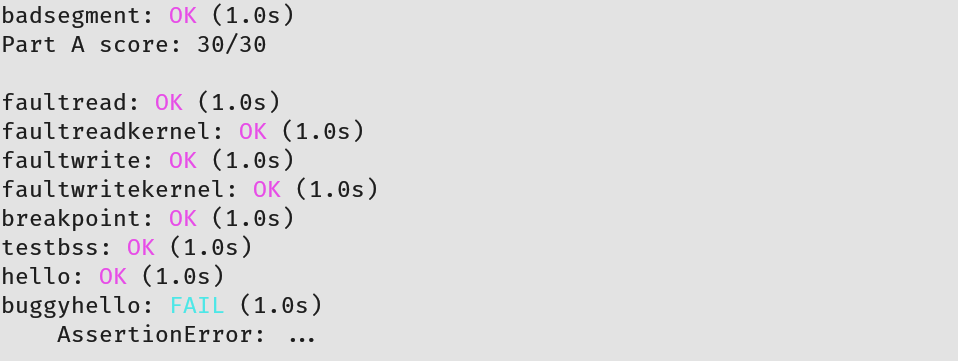
\includegraphics[width=0.8\linewidth]{lab3/exercise8_1.png}
        \caption{程序通过hello测试}
        \label{fig:lab3/exercise8_1}
    \end{figure}
\end{exerciseSolution}

\subsection{Page faults and memory protection}
\par 内存保护是操作系统的一个非常重要的特性,能够保证bug不能够损坏其他的程序或者操作系统。操作系统通常依赖于硬件来完成这一功能。操作系统能够让硬件知道那笑虚拟地址是有效的。当程序尝试访问一个无效地址或者越权操作时就会触发异常。如果异常是可以修复的,那么就会修复异常并继续运行程序,否则就不会继续运行。
\par 在许多操作系统中,内核在初始情况下只会分配一个内核堆栈。如果程序想要访问这个堆栈之外的堆栈空间,就会触发异常,内核会自动分配页个程序然后继续让程序运行。
\par 但是系统调用需要存在问题,大部分系统系统调用接口让用户传递一个指向用户缓冲区的指针给内核,但是:
\begin{enumerate}
    \item 内核中的page fault比用户中的page fault严重。如果内核出现page fault,那么这是内核bug,而且异常处理会中断内核的执行。但是当内核解引用用户程序的时候,它需要一种方法标记这些page fault确实是由用户引起的。
    \item 内核通常比用户程序由更高级别的权限。用户程序可能会传递一个内核可读写但是用户不行的指针。此时内核不能对其进行解引用,否则可能泄露内核信息。
\end{enumerate}

\begin{exerciseEnv}{9}
    \par 修改kern/trap.c,使其能够检测内核模式下的page fault发生并发出kernel panic。阅读kern/pmap.c中的use\_mem\_assert并实现其中的use\_mem\_check。修改ker/syscall.c检查输入参数。
    \par 启动内核并运行user/buggyhello。环境应该被摧毁,但是不应该出现kernel panic。应该能够看到:
    \inputCodeSetLanguage{bash}
    \begin{lstlisting}[numbers=none]
[00001000] user_mem_check assertion failure for va00000001
[00001000] free env 00001000
Destroyed the only environment - nothing more to do!
    \end{lstlisting}
    \par 最后,修改kern/kdebug.c中的debuginfo\_eip来运行user\_mem\_check检查use, stabs和stabstr。如果现在运行user/breakpoint,应该能够从内核监视器中运行backtrace来检查在page fault之前检查lib/libmain.c。是什么导致了page fault?
\end{exerciseEnv}

\begin{exerciseSolution}{9}
    \par 首先检查page fault是否在内核模式,即检查Trap Frame中的tf\_cs,在page\_fault\_handler中添加的代码如下:
    \inputCodeSetLanguage{c}
    \begin{lstlisting}
if(tf->tf_cs == GD_KT)
    panic("page_fault_handler: kernel page fault");
    \end{lstlisting}
    \par pmap.c中的user\_mem\_check。阅读user\_mem\_assert, 可以发现它调用了user\_mem\_check。然而user\_mem\_check的功能当前永辉态程序是否有对于$[va, va+len)$的perm|PTE\_P的访问权限。因此在user\_mem\_check中查看用户态程序中的页表项,然后检查其perm|PTE\_P。最终实现的程序如下:
    \begin{lstlisting}
int user_mem_check(struct Env *env, const void *va, size_t len, int perm) {
    uint32_t start = (uint32_t)ROUNDDOWN(va, PGSIZE);
    uint32_t end = (uint32_t)ROUNDUP(va + len, PGSIZE);
    pte_t *page;
    for (; start < end; start += PGSIZE) {
        page = pgdir_walk(env->env_pgdir, (void *)start, 0);
        if (!page || start > ULIM || ((uint32_t)(*page) & perm) != perm ) {
            if (start <= (uint32_t)va)
                user_mem_check_addr = (uintptr_t)va;
            else
                user_mem_check_addr = (uintptr_t)start;
            return -E_FAULT;
        }
    }
    return 0;
}
    \end{lstlisting}
    \par 接下来对于kern/syscall.c进行补全。通过观察发现需要补全的是sys\_cputs函数。通过注释可以发现需要用户程序检查用户对于虚拟地址空间$[s, s+len)$是否具有访问权限,而这个则可以用上面实现的user\_mem\_assert实现。这个函数补全后如下:
    \begin{lstlisting}
static void sys_cputs(const char *s, size_t len) {
    user_mem_assert(curenv, s, len, 0);
    cprintf("%.*s", len, s);
}
    \end{lstlisting}
    \par 最后修改kern/kdegbug.c中的debuginfo\_eip。添加如下代码:
    \begin{lstlisting}
if(user_mem_check(curenv, usd, sizeof(struct UserStabData), PTE_U))
    return -1;
    \end{lstlisting}
    \par 运行make run-breakpoint,显示如图\ref{fig:lab3/exercise9_1}所示。可以看到,输入backtrace能够显示backtrace之前能够追踪进入libmain.c
    \begin{figure}[htb]
        \centering
        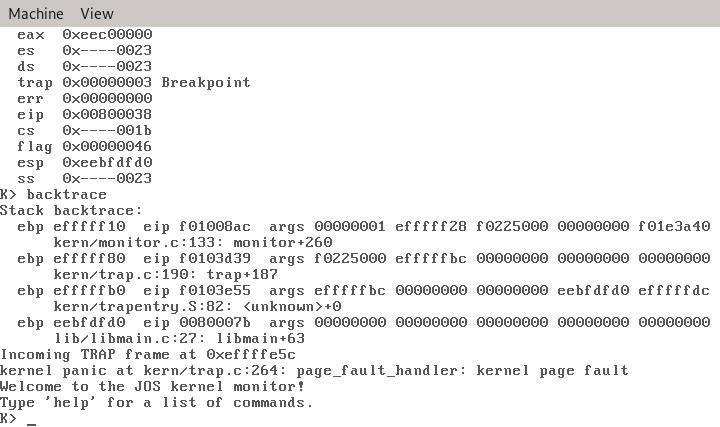
\includegraphics[width=0.7\linewidth]{lab3/exercise9_1.png}
        \caption{运行user/breakpoint后的结果}
        \label{fig:lab3/exercise9_1}
    \end{figure}
    \par 通过gdb进行追踪,发现是由于执行mon\_backtrace时进行追踪时到达了用户栈顶,然后在打印参数时访问的第六个参数超过了用户栈的大小,如图\ref{fig:lab3/exercise9_2}所示。
    \begin{figure}[htb]
        \centering
        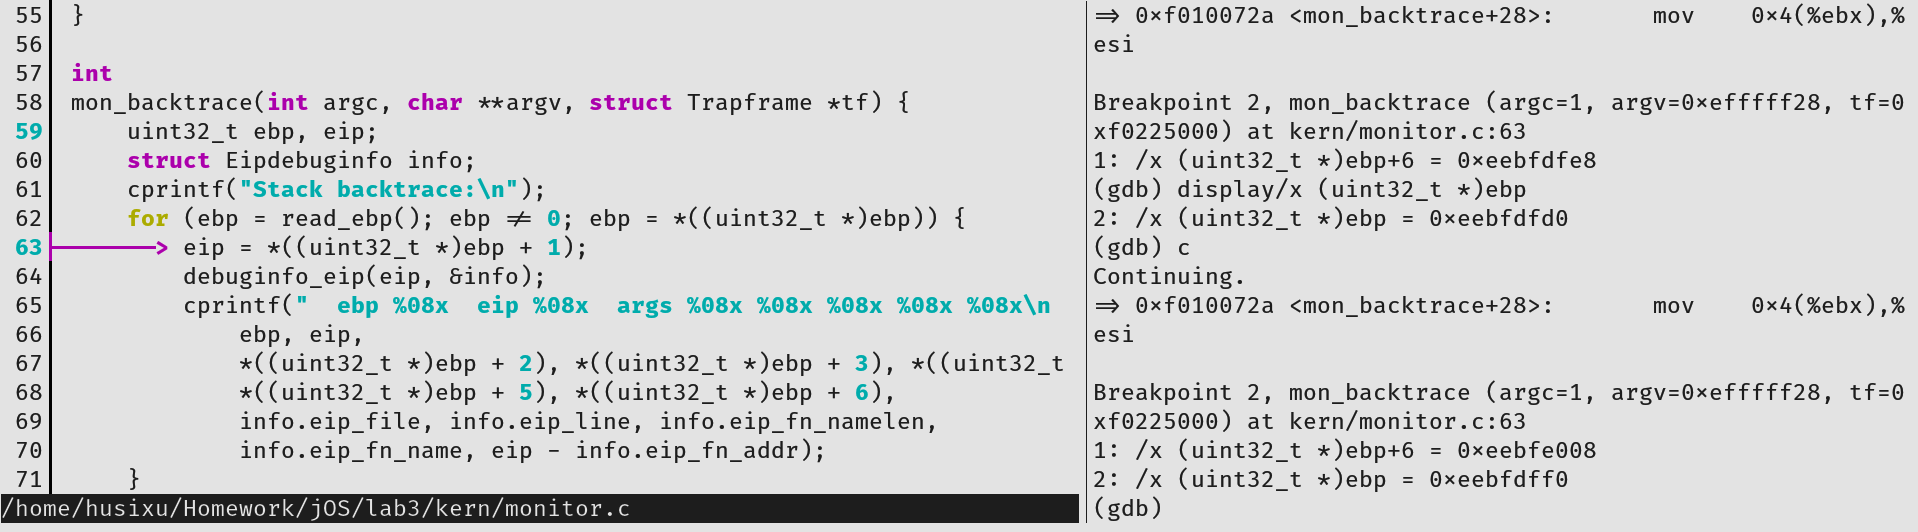
\includegraphics[width=0.9\linewidth]{lab3/exercise9_2.png}
        \caption{使用gdb进行追踪}
        \label{fig:lab3/exercise9_2}
    \end{figure}
    \par 最后,使用make grade 进行测试,发现能够正常通过所有测试,如图\ref{fig:lab3/exercise9_3}所示。
    \begin{figure}[htb]
        \centering
        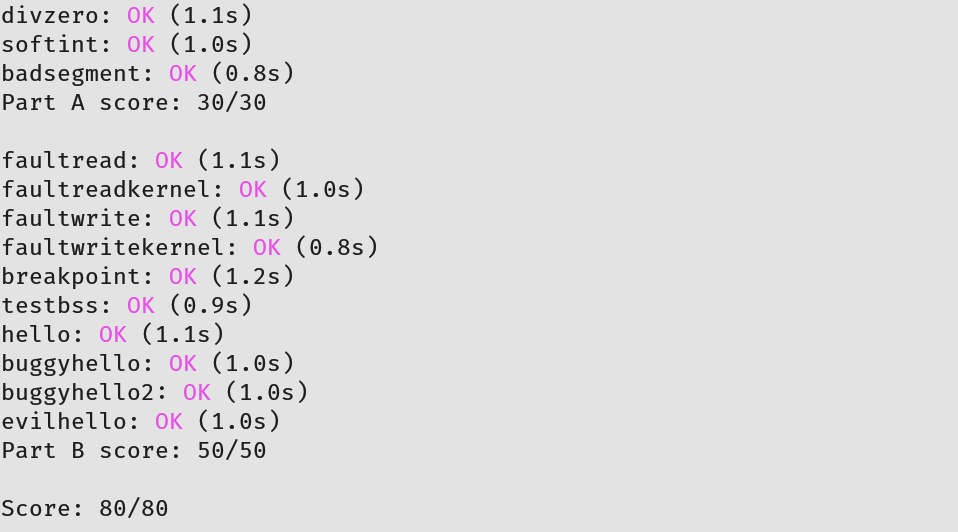
\includegraphics[width=0.6\linewidth]{lab3/exercise9_3.png}
        \caption{make grade通过所有测试}
        \label{fig:lab3/exercise9_3}
    \end{figure}
    \FloatBarrier
\end{exerciseSolution}

\begin{exerciseEnv}{10}
    \par 启动你的内核并运行user/evilhello。环境应该被摧毁并且内核不应该panic。你应该能够看到:
    \inputCodeSetLanguage{bash}
    \begin{lstlisting}[numbers=none]
[00000000] new env 00001000
...
[00001000] user_mem_check assertion failure for va f010000c
[00001000] free env 00001000
    \end{lstlisting}
\end{exerciseEnv}
\begin{exerciseSolution}{10}
    \par 运行evilhello,结果如图\ref{fig:lab3/exercise10_1}所示。环境被摧毁且没有发生kernel panic。
    \begin{figure}[htb]
        \centering
        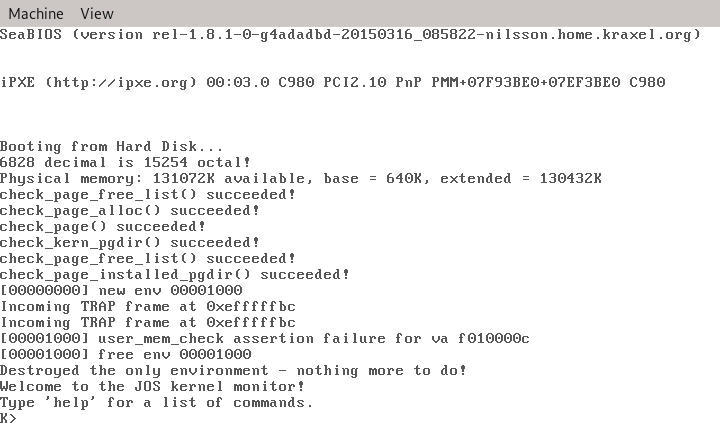
\includegraphics[width=0.6\linewidth]{lab3/exercise10_1.png}
        \caption{evilhello运行结果}
        \label{fig:lab3/exercise10_1}
    \end{figure}
    \FloatBarrier
\end{exerciseSolution}


